\section{Two-option contrasts and the sharp position designs}
\label{app:general-position}
Throughout this appendix $n$ counts options and $N$ counts questions.
An order $\pi$ maps display slots to option labels. Consider the
$m=n(n-1)$ ordered pairs of distinct slots occupied by options 0 and 1.
The full-order population is uniform on these pairs. In a Latin block
each of the $n$ observed pairs is distinct, and each slot occurs once in
each coordinate. The centered weight matrix $e$ consequently vanishes
on the diagonal and has zero row and column sums. Its squared norm is
$1/n-1/m$. The space $V$ of matrices with these constraints has
dimension $d_0=m-(2n-1)$. Indeed, a linear dependence among the row and
column equations requires $a_i+b_j=0$ whenever $i\ne j$, which forces
all $a_i$ equal and all $b_j$ their negatives. For a centered matrix
$h$, its variance over orders is $\|h\|^2/m$, so its normalized risk
is $m\,\mathbb E(e^\top h)^2/\|h\|^2$, with matrices viewed as vectors.
The operator $m\mathbb E[ee^\top]$ has trace $n-2$. Every independent
extra dyad function integrated in each block removes one dimension
after projection onto $V$, proving the real-score bound of
Section~\ref{sec:theory}.

\paragraph{Why the trace bound holds for correctness.}
Write $V=V_s\oplus V_a$ for the symmetric and skew-symmetric parts.
They have dimensions $s=n(n-3)/2$ and $a=(n-1)(n-2)/2$. For symmetric
edge weights the $n$ row equations are independent since $c_i+c_j=0$
for every edge forces $c_i=0$. For skew edge weights their rank is $n-1$.
In $V_s$ assign alternating signs to both directions of the edges of a
four-cycle and zero elsewhere. In $V_a$ assign $+1$ around a triangle,
$-1$ in the opposite direction and zero elsewhere. For either witness
$h$, uniformly permute its slot labels, and consider
$F=\mathbb E[hh^\top/\|h\|^2]$. This operator is supported on the
corresponding subspace and has trace one.

On symmetric edge weights its coefficients depend only on whether two
unordered edges coincide, share a vertex, or are disjoint. At edge
$ij$ the sum on neighboring edges is $-2h_{ij}$ for every $h\in V_s$,
and the sum on disjoint edges is $h_{ij}$. Thus $F$ acts as a scalar
on $V_s$. In the skew case, exchanging the endpoints of a disjoint
edge forces its coefficient to vanish. At $ij$ the remaining
off-diagonal term is proportional to
$\sum_{t\ne i,j}(h_{it}-h_{jt})=-2h_{ij}$, again giving a scalar.
The two operators are therefore the corresponding orthogonal
projectors divided by $s$ and $a$. Selecting the two witnesses with
probabilities $s/d_0$ and $a/d_0$ gives $\mathbb E[hh^\top/\|h\|^2]
=P_V/d_0$. For every block the resulting mean normalized squared
error is $m\|e\|^2/d_0=(n-2)/d_0$. Taking the design expectation
proves Theorem~1 for correctness differences without a symmetry
assumption on the design.

\paragraph{General position-balanced budgets.}
Let $k$ be a positive multiple of $n$ with $k\le n!$, and let
$c_j$ count how often the two distinguished options occupy slot dyad
$j$ in a block. The weight errors $e_j=c_j/k-1/m$ still have zero
row and column sums. The same two ternary witnesses have conditional
mean normalized squared error $m\|e\|^2/d_0$ for each block. With
$h=k\bmod m$, the minimum of $\sum_j(c_j-k/m)^2$ over nonnegative
integer counts of sum $k$ is $h(m-h)/m$. Moving one count from a
cell to a cell smaller by at least two strictly decreases the sum,
so a minimizing vector has $h$ entries $\lceil k/m\rceil$ and all
others $\lfloor k/m\rfloor$. Applying this lower bound to every
feasible block gives the multi-budget bound in the main text.

\paragraph{Recovering the two risks from swaps.}
Randomly select the two distinguished semantic labels as well as the
slot relabeling of the witness. For two rows $x,y$, the ordered slot
dyad in $x$ is then uniform and the corresponding dyad in $y$ follows
by applying $y^{-1}x$. The inner product of a unit witness with its
image, averaged over slot relabelings, is the trace of this permutation
on $V_s$ or $V_a$ divided by the corresponding dimension, by the frame
identity above. With $x=y$ the ratio is one. With $x\ne y$ their
relative permutation is a derangement. If it has $u$ two-cycles, it
fixes $u$ unordered edges, exchanging their endpoints. Thus its trace
on all symmetric edges is $u$, and on all skew edges it is $-u$.
The symmetric vertex effects $b_i+b_j$ form the vertex permutation
representation, with trace zero on a derangement. The skew vertex
effects $b_i-b_j$ remove the constant vertex representation, giving
trace $-1$. Subtraction leaves traces $u$ and $1-u$ on $V_s$ and
$V_a$. The diagonal pairs have weight $1/n$ in the block square.
The other pairs give the two terms in Eq.~\eqref{eq:swaps}. Randomizing
the witnesses in this argument is valid even for families that are
not closed under slot relabeling.

With unrestricted distinct orders, symmetrizing a design over all
permutations of the $n!$ population indices preserves each contrast
class and yields simple random sampling. Its common risk ratio is
$(n!-n)/(n(n!-1))<1/n$. In contrast, $L_n=1/n+(n-1)/(nd_0)>1/n$.

\paragraph{Sharp upper bounds from explicit samplers.}
At each $n$ in Table~\ref{tab:template-weights}, select a template $T$
with the indicated probability. Independently shuffle its columns and
relabel its symbols uniformly, using the same resulting rows for both
models. Every displayed order has the required marginal. All template
rows are specified in \texttt{position-templates.json}. For example
the two six-row templates, written from the top down, are
\[
\begin{split}
T_1&=(012345,103254,240513,351402,425130,534021),\\
T_2&=(012345,103452,231504,345120,450231,524013).
\end{split}
\]
For templates of any size, the following calculation tests a proposed
mixture on \emph{all} real score vectors. For rows $x,y$ of $T$, two
uniform relabelings $g,h$ give the pair $(gxh,gyh)$, whose relative
permutation is $h^{-1}x^{-1}yh$. Conditional on this relative
permutation, the first row is uniform. The resulting quadratic form
under the uniform population inner product is thus a central
convolution. On the component indexed by partition $\lambda\vdash n$,
its eigenvalue before centering is
\begin{equation}
 \rho_\lambda=\frac{1}{n^2 f_\lambda}
 \sum_T w_T\sum_{x,y\in T}\chi_\lambda(x^{-1}y),
 \qquad f_\lambda=\chi_\lambda(1).
 \label{eq:character-certificate}
\end{equation}
Indeed, averaging the representation over a conjugacy class gives a
scalar matrix by Schur's lemma, and its trace determines the scalar
\citep{diaconis1981}. Centering removes the trivial component. The
largest remaining value is the real worst-case ratio. The certificate
uses integer characters, rational weights and checks all nontrivial
partitions. For each $n$ the components $(n-2,2)$ and $(n-2,1,1)$
reach the displayed maximum. Exhibiting a sampler and matching the
universal lower bound proves optimality without listing all Latin
squares of these orders.

\begin{table}[ht]
\centering
\caption{Probability of choosing each template before independent
uniform relabeling of slots and options. These are sharp upper certificates.}
\label{tab:template-weights}
\begin{tabular}{rrrr}
\toprule
$n$ & $w_1$ & $w_2$ & Largest centered eigenvalue \\
\midrule
6 & $20/133$ & $113/133$ & $4/19$ \\
7 & $25/29$ & $4/29$ & $5/29$ \\
8 & $17/41$ & $24/41$ & $6/41$ \\
9 & $37/55$ & $18/55$ & $7/55$ \\
10 & $58/71$ & $13/71$ & $8/71$ \\
\bottomrule
\end{tabular}
\end{table}

\section{Connectivity and quantitative adjacency certificates}
\label{app:connectivity}
If $X$ is a uniform row of a random block, the uniform order marginals
give $X\sim\mathrm{Unif}(S_n)$. For every profile,
\[
 v(d)=\operatorname{Var}(\mathbb E[d(X)\mid B])
      +\mathbb E\operatorname{Var}(d(X)\mid B).
\]
The first term is the risk of the sample mean before normalization.
On the centered unit sphere, equality with $v(d)$ occurs exactly when
the second term vanishes, meaning $d$ is constant on every block of
positive mass. A component indicator gives equality for every law if
the allowed graph is disconnected. If the graph is connected, uniform
sampling over the allowed blocks has full support and uniform marginals
by transitivity. Equality would force $d$ to be constant on all orders.
The maximum on the centered unit sphere is attained, so this law has
worst-case risk strictly below one. Substituting a cut indicator gives
Eq.~\eqref{eq:cut}. For the group formulation, left multiplication by
$x^{-1}$ takes any allowed block containing $x$ to a block containing
the identity. Consequently the neighbors of $x$ are $xu$, where $u$
ranges over the nonidentity rows of normalized blocks. Reachability
from $x$ is precisely its left coset of the subgroup generated by the
rows. This proves Theorem~2.

At six options the two reduced row-complete blocks are
\[
\begin{split}
B_1&=(012345,130524,204153,351402,425031,543210),\\
B_2&=(012345,135024,251403,304152,420531,543210).
\end{split}
\]
For every row $x$ here, $x(i)+x(5-i)=5$ for all zero-based slots $i$.
Under a common relabeling $g$, all rows of $gB$ therefore give the
same matching of options across opposite slots. The subgroup closure
has 24 elements. A direct enumeration at four, five and six options
generates respectively 4, 56 and 9,408 reduced Latin squares. Maximum
adjacency retains 1, 9 and 2, with subgroup orders 4, 120 and 24.

For eight, nine and ten options we use the published exhaustive
row-complete catalogues of \citet{wanlesscatalogue} (12, 12 and 492
reduced squares). Seven has no row-complete square. For a displayed
template $T$, let $q_x(i)$ be the slot of symbol $i$ in row $x$.
For a centered ternary dyad witness $h$, the normalized risk averaged
over uniform option relabelings is
\[
 U_T(h)=
 \frac{\sum_{i\ne j}\big(\sum_{x\in T}h(q_x(i),q_x(j))\big)^2}
      {n^2\sum_{u\ne v}h(u,v)^2}.
\]
The numerator enumerates the two distinguished semantic options under
the random label map. The certificate specifies six, four and six
weighted signed cycles or triangles at the respective sizes.
Direct integer evaluation gives
$\min_T\sum_h w_h U_T(h)=69/280,\ 43/243,\ 12427/99080$.
We round the final lower bound down to $1/8$ in the main table.
These statements use the completeness of the cited catalogue. For the
strict upper bounds it suffices to exhibit, respectively, two, one and
two row-complete templates whose rows generate $S_n$. In each case
the verifier exhibits a transposition and checks transitivity on
ordered pairs of distinct slots. Every transposition is then a
conjugate within the generated group. No catalogue completeness
assumption enters the upper bounds.
\section{An infinite family attaining the position bound}
\label{app:two-prime}
Let $n=2p$ with $p$ an odd prime. Put $s=n(n-3)/2$,
$a=(n-1)(n-2)/2$, $d=s+a=n^2-3n+1$, and $t=s/d<1/2$.
Choose the cyclic addition table of $\mathbb Z_n$ with probability
$w=t(n-1)/p$ and the following square otherwise. Both probabilities are positive.
In the second square, slots and symbols belong to $\mathbb F_p\times\{0,1\}$.
The $2p$ rows are the following maps, with $i\in\mathbb F_p$ and
the first coordinate calculated modulo $p$:
\[
\begin{aligned}
 A_i(x,c)&=(x+(-1)^c i,c),\\
 B_i(x,c)&=(x+(-1)^c i+c,1-c).
\end{aligned}
\]
Each row permutes the symbols. For a fixed slot, the two row families
range once over opposite fibers, proving the Latin property. Independently
permute slots and symbols uniformly after choosing the square.

\paragraph{Relative rows.}
Condition on two distinct uniformly drawn rows. Within either fiber
of row indices, the relative row translates both copies of $\mathbb F_p$
by nonzero increments, so its cycle type is $(p,p)$.
Across fibers, $A_i^{-1}B_j$ interchanges the copies and adds
$(-1)^c(i+j)+c$ to the first coordinate. Squaring adds one on both
copies, so the relative row is a single $2p$-cycle. In the cyclic
table a nonzero translation is equally likely to be any of the
$n-1$ increments. Exactly one increment yields $p$ transpositions,
and $p-1$ yield each long-cycle type. Thus in the mixture the probability
of type $2^p$ is $w/(n-1)=t/p$, the expected number of transpositions
in the cycle decomposition is $t$, and the mean sign is $-1/(n-1)$.
Indeed the probability of an even relative row in either table is
$(p-1)/(2p-1)$.

\paragraph{The low-dimensional components.}
By Eq.~\eqref{eq:character-certificate}, it suffices to bound the
off-diagonal mean character divided by degree by $1/d$ on every
nontrivial irreducible. The symmetric and skew dyad components have
dimensions $s,a$ and mean characters $t,1-t$, giving equality in
both. On a derangement with $u$ transpositions their characters are
$u,1-u$. Every row pair with $u>0$ has negative sign. The two
sign twists therefore have mean characters $-t,t-1/(n-1)$, giving
ratios at most $1/d$ since $t<1-t$. The sign character and standard
character have negative means. The sign twist of the standard character
has ratio $1/(n-1)^2<1/d$.

\paragraph{All remaining components, uniformly in the prime.}
For $n\ge256$, the low-degree classification of Rasala
\citep{rasala} gives degree $f\ge n(n-1)(n-5)/6\ge n^3/7$
after removing the trivial representation and the seven nontrivial
components treated above. On an $n$-cycle the absolute character is
at most one by the Murnaghan--Nakayama rule. On $(p,p)$ it is at
most two: in a beta-set encoding each removable $p$-hook moves one
bead to a vacant position $p$ places lower. All initially available
moves have disjoint endpoints and can be executed together. Three
moves would remove $3p$ boxes from a shape of size $2p$. After
the first move the absolute character on the remaining $p$-cycle is
at most one. On $2^p$ the Fomin--Lulov inequality \citep{fominlulov}
gives absolute character at most
\[
 \frac{2^p p!}{\sqrt{(2p)!}}\sqrt f\ \le\ (2n)^{1/4}\sqrt f .
\]
Here $\binom{2p}{p}\ge4^p/\sqrt{4p}$ follows by induction from $p=1$.
Since $t/p<1/n$, the absolute off-diagonal ratio on all these components
is at most
\[
 \frac{2}{f}+\frac{(2n)^{1/4}}{n\sqrt f}
 \le \frac{1}{n^2}\left(\frac{14}{n}+
          \frac{2^{1/4}\sqrt7}{n^{1/4}}\right)<\frac1{n^2}<\frac1d.
\]
The parenthesis is less than one already at 256 and decreases.
Adding back the diagonal gives largest centered eigenvalue
$1/n+(n-1)/(nd)=L_n$. Theorem~1 supplies the matching correctness
lower bound. This proves simultaneous optimality for every prime
$p\ge131$, without a separate search at each size.

\section{An exact attainment criterion and the twelve-option certificate}
\label{app:attainment}
For $n\ge4$, let $D=n^2-3n+1$ and let $\mathcal C$ be the set of
derangement cycle types in $S_n$. For a Latin square $T$, draw two
distinct rows $x,y$ uniformly and put $q_T(C)=\Pr(x^{-1}y\in C)$.
Let $Q_n$ be the convex hull of these histograms over Latin squares of
order $n$. Repeated histograms need only be included once.

\paragraph{Cycle-type criterion.}
The bound $L_n$ is attained simultaneously for real scores and
correctness differences if and only if there exists $q\in Q_n$ with
\begin{equation}
 \sum_{C\in\mathcal C} q(C)\chi_\lambda(C)
 \ \le\ f_\lambda/D \qquad(\lambda\vdash n,\ \lambda\ne(n)).
 \label{eq:attain-lp}
\end{equation}
These are rational linear feasibility constraints: write
$q=\sum_T w_Tq_T$, $w_T\ge0$, $\sum_Tw_T=1$.
Whenever feasible, at most $|\mathcal C|$ templates with rational
weights suffice. In particular this test uses cycle types of row
pairs rather than all $n!$ coordinates of a response. A restricted
list suffices to prove attainment; an infeasibility claim requires
control of all eligible histograms.

\emph{Proof.} Average a feasible design independently over option
and slot relabelings. This preserves the uniform marginals. Each
relabeling merely permutes the coordinates of a profile, so the
worst-case risk cannot increase in either profile class. After
averaging, the design selects a template and applies two uniform
relabelings. Conversely, every point in $Q_n$ is realized in this way.
The nonconstant eigenvalues in Eq.~\eqref{eq:character-certificate}
are $1/n+(n-1)\sum_C q(C)\chi_\lambda(C)/(nf_\lambda)$.
Comparing these values with $L_n=1/n+(n-1)/(nD)$ gives
Eq.~\eqref{eq:attain-lp} in both directions for real profiles.
The lower bound already has a correctness witness, so a feasible
solution is sharp for both classes. A rational feasible polytope
has a rational vertex. Its histogram lies in a simplex spanned by
affinely independent template histograms, at most $|\mathcal C|$
of them since their entries sum to one. Its barycentric coordinates
in that simplex are rational.

The dual form gives a certificate of impossibility. Define
$b_{T\lambda}=\sum_Cq_T(C)\chi_\lambda(C)/f_\lambda-1/D$ for
nontrivial $\lambda$. The criterion fails precisely when there is a
probability vector $u$ on these partitions such that
$\sum_\lambda u_\lambda b_{T\lambda}>0$ for every template.
Indeed the convex hull of the finite row vectors $b_T$ then misses
the closed negative orthant. Strict separation supplies a nonzero
nonnegative normal (otherwise its supremum on the orthant is infinite);
normalizing its sum gives $u$. Conversely such a $u$ excludes every
feasible mixture.

\paragraph{What balance is necessary?}
The two dyad inequalities have respective left sides $t$ and $1-t$,
where $t=\sum_Cq(C)m_2(C)$ and $m_2(C)$ counts transpositions in the
cycle decomposition. Their right sides are $s/D$ and $a/D$ with
$s+a=D$. Hence both must be equalities. This gives an initial scalar
test before the other inequalities. The same equality is necessary
even for correctness alone by Eq.~\eqref{eq:swaps}. For an exact
criterion for that class alone, replace $\chi_\lambda(C)/f_\lambda$
in the normalized inequalities by
\[
 h_z(C)=\mathbb E_{x,g}[z(x)z(xg)]/\mathbb E_x[z(x)^2]
\]
for each centered nonconstant ternary profile $z$ (center after
choosing the ternary entries), with independent uniform $x\in S_n$
and $g\in C$. Indeed the off-diagonal normalized second moment is
then $\sum_Cq(C)h_z(C)$; the diagonal contribution is unchanged.
These are again finitely many rational inequalities, though generally
far more numerous.

\paragraph{Screening the remaining degrees.}
For a candidate $q$, put $H(q)^2=\sum_C q(C)^2 n!/|C|$.
Column orthogonality gives
$\sum_\lambda(\sum_Cq(C)\chi_\lambda(C))^2=H(q)^2$.
Thus all components of degree at least $DH(q)$ satisfy the test
automatically. This bound can shorten an exact check without
assuming that the two dyad components are the worst ones.

\paragraph{Twelve options.}
The two squares in \texttt{certificates/position-templates.json}
under key \texttt{12} have total transposition counts 54 and 27 over
their 66 unordered row pairs. Draw the first square with probability
$23/109$ and the second with probability $86/109$, then shuffle
symbols and slots independently. The mean transposition count is
$(23\cdot54+86\cdot27)/(109\cdot66)=54/109=s/D$.
For this histogram $186<109H(q)<187$, so degrees at least 187 are
automatically covered. The accompanying exact certificate checks all
76 nontrivial partitions. The largest normalized risk is $10/109$
on $(10,2)$ and $(10,1,1)$; the largest remaining value is
$1873/21582<10/109$. One verifier uses the Murnaghan--Nakayama rule;
a second expands the Frobenius character formula and recomputes the
pair types from the rows. By the criterion and the correctness lower
bound, $10/109$ is the exact optimum for both classes.


\section{Sharp four-option risks across sampling budgets}
\label{app:budgets}

\paragraph{A binary certificate for finite populations.}
Let there be $M$ possible orders, and let $\mathcal B$ be a nonempty
family of allowed $k$-subsets, $0<k<M$. A design samples an equally
weighted block with order inclusion probabilities $k/M$. For
$b_B=\mathbf 1_B$ write $u_B=(b_B-(k/M)\mathbf 1)/\sqrt{k(1-k/M)}$,
$W=\mathrm{span}\{u_B:B\in\mathcal B\}$, $r=\dim W$ and $T=M/k-1$.
Suppose a feasible design $D_*$ satisfies the weighted finite tight
frame identity $\mathbb E_{A\sim D_*}u_Au_A^\top=P_W/r$, where
$P_W$ is the orthogonal projector \citep{benedetto2003}. Its normalized
worst-case risk is $T/r$ for real profiles and for differences of
binary correctness indicators.

For any nonconstant $d$, let $z$ be its centered vector divided by its
Euclidean norm. The squared error of a realized block divided by
the full-order variance is $T\langle u_B,z\rangle^2$. For $D_*$,
averaging over $B$ gives $(T/r)\|P_Wz\|^2$, which proves the upper
bound. For the lower bound, take an independent $A\sim D_*$ and
assign model A the correctness vector $\mathbf 1_A$ and model B the
zero vector. The normalized centered profile is $u_A$. For every
feasible $B$, the average normalized squared error over $A$ is
$T u_B^\top(P_W/r)u_B=T/r$. Averaging over any candidate design on
$B$ leaves this value unchanged. Some fixed binary profile must
therefore realize risk at least $T/r$ for that design. The argument
allows the competing design to use arbitrary weights on its feasible blocks.

\paragraph{Enumeration and exact matrices.}
Index the 24 \emph{display} orders lexicographically, using four labels
numbered from zero. For a position-balanced $k$-block, each label
appears first $k/4$ times. Enumerate all choices of $k/4$ of the six
rows starting with each label, take their union and test the remaining
position, precedence and directed-adjacency counts. At $k=8$ this
gives 255, 99 and 15 feasible blocks in the three nested classes. At
$k=12$ it gives 640, 180 and 22. For each template draw a uniform
option relabeling. For position balance also permute slots uniformly.
For precedence and adjacency keep the slots or reverse them with equal
probability. The eight-call attaining mixtures are explicit in
Table~\ref{tab:eight-templates}. The twelve-call templates are given
in the accompanying machine-readable certificate.

\begin{table}[h]
\centering
\caption{Eight-call samplers. Each tuple lists the lexicographic indices of the eight displayed rows
before random relabeling. A uniform pair of distinct Williams blocks is an equivalent full-adjacency sampler.}
\label{tab:eight-templates}
\begin{tabular}{llr}
\toprule
Balance & Template & Selection probability \\
\midrule
Position & $(0,1,8,9,16,17,18,19)$ & $6/7$ \\
         & $(0,3,7,11,12,16,20,23)$ & $1/7$ \\
Position and precedence & $(0,1,6,10,13,17,22,23)$ & $2/11$ \\
         & $(0,2,7,10,13,17,21,22)$ & $2/11$ \\
         & $(0,3,7,11,12,16,20,23)$ & $1/11$ \\
         & $(0,3,7,11,14,17,18,22)$ & $6/11$ \\
All three & $(0,1,8,10,13,17,19,23)$ & $4/5$ \\
         & $(0,2,7,10,13,16,21,23)$ & $1/5$ \\
\bottomrule
\end{tabular}
\end{table}

For each attaining law form the rational matrix
$C=(M/k^2)\mathbb E[b_B b_B^\top]-\mathbf1\mathbf1^\top/M$.
The verifier checks its marginals, its trace $T$, the identity
$C^2=\lambda C$ and $Cu_B=\lambda u_B$ for \emph{every feasible}
block in the corresponding class. The range of $C$ lies in $W$
because $C=T\mathbb E[u_Bu_B^\top]$. The final check makes its range
equal to $W$. Hence $C=\lambda P_W$ and
$r=T/\lambda$. In increasing order of constraints the resulting ranks
are $(14,11,5)$ at eight and $(14,11,6)$ at twelve. The binary
certificate proves optimality in both profile classes. Simple random
sampling has constant risk $(M-k)/(k(M-1))$ on centered profiles.
Symmetrizing any unrestricted candidate over population relabelings
gives this law, proving the unrestricted lower bound for correctness
as well.

The complement of a balanced $k$-block satisfies the corresponding
constraints at $24-k$. The two centered sample means differ by the
factor $-k/(24-k)$ since their weighted sum is zero. This bijection
preserves uniform marginals and scales every profile risk by
$k^2/(24-k)^2$. It transfers the four- and eight-call optima to
20 and 16 calls. At 24 the target is observed exactly.

\paragraph{How the full-adjacency sampler changes with budget.}
The six four-call Williams blocks partition the population. Their
15 pairwise unions exhaust the admissible eight-call blocks, with
probability $1/15$ per union in the certified sampler. Writing the six
block means as a population of size six, the finite population
correction for sampling two distinct means is $(6-2)/(2(6-1))=2/5$.
At twelve calls there are also the even and odd permutation halves.
An attaining sampler selects a uniform triple of Williams blocks
with probability $5/6$ and a uniform parity half with probability $1/6$.
The two added blocks supply the sixth residual direction.

At eight calls, position features together with the constant have
rank ten, and precedence raises that rank to thirteen. Exact rational
elimination gives these ranks. The complementary dimensions match
the frame ranks 14 and 11. For full balance, every centered feasible
block is constant on each of the six Williams groups, a centered space
of dimension five. Hence the two projections of
Section~\ref{sec:budget} are precisely onto the two feasible-block
spans. For item $i$, the squared-error expectation equals
$d_i^\top C d_i/24$. Summing across independent items gives
Eq.~\eqref{eq:residual-threshold}.

\section{Replaying fixed-budget risks from the 24-order profiles}
\label{app:eight-replay}

The target is the difference of mean accuracies averaged over all 24
orders. For each question we compress the paired full-order correctness
difference into its positive and negative order masks. Questions with
identical masks are counted within stratum. These anonymous histograms
suffice for point risks and the paired item bootstrap. The three
matched panels use Qwen2.5-3B-Instruct and SmolLM3-3B. The separate
6,144-question HellaSwag comparison uses Qwen2.5-1.5B-Instruct and
Granite-3.3-2B-Instruct. It shares 227 questions with the matched
HellaSwag panel. We report it separately throughout.

For each block the integer score is the number of its positive
orders minus its number of negative orders. At $k=4,8$ the item
loss is $((24/k)\,\mathrm{score}-\sum_\pi d_i(\pi))^2/576$.
The replay sums the loss against the exact rational support weights.
As a second calculation at eight calls, it projects every item
using integer orthogonalization of position and precedence features
and the six Williams-group means. Both calculations agree exactly on
all balanced item risks, and the four-call risks and full-order gaps
match the earlier releases.

\begin{table}[h]
\centering
\caption{Conditional MSE of the paired accuracy gap in units of $10^{-6}$.
The first three columns use 992 questions each. The final column uses the separate smaller-model HellaSwag cohort.}
\label{tab:eight-all}
\begin{tabular}{@{}llrrrr@{}}
\toprule
Calls & Design & HellaSwag 3B & MMLU 3B & LogiQA 3B & HellaSwag 1.5B/2B \\
\midrule
4 & Unrestricted distinct        & 79.836 & 65.745 & 63.033 & 8.490 \\
4 & Position minimax             & 22.125 & 21.377 & 21.629 & 4.713 \\
4 & Precedence minimax           & 21.592 & 20.181 & 20.091 & 4.640 \\
4 & Williams                     & 21.645 & 20.869 & 19.625 & 4.586 \\
\midrule
8 & Unrestricted distinct        & 31.934 & 26.298 & 25.213 & 3.396 \\
8 & Position minimax             & 8.493 & 8.170 & 8.297 & 1.810 \\
8 & Precedence minimax           & 8.018 & 7.611 & 7.720 & 1.730 \\
8 & Two distinct Williams blocks & 8.658 & 8.348 & 7.850 & 1.834 \\
8 & Two disjoint position blocks & 8.773 & 8.477 & 8.565 & 1.870 \\
8 & Two disjoint precedence blocks & 8.328 & 7.879 & 7.887 & 1.798 \\
8 & Rotations and reversals      & 7.837 & 8.437 & 9.082 & 1.702 \\
\bottomrule
\end{tabular}
\end{table}

The disjoint-pair baselines choose uniformly among disjoint pairs
from the corresponding four-call minimax sampler. At eight calls
these baselines have worst-case ratios $1/6$, $3/14$ and $2/5$
for position, precedence and full adjacency, respectively. For the
rotation baseline we randomly relabel the four forward rotations and
their four reversed orders \citep{khan2026} per question. This law
partitions the population into three equiprobable blocks. A binary
profile constant on each block attains worst-case ratio one. It gives
the lowest observed point MSE among the tested eight-call designs on
both HellaSwag cohorts (Table~\ref{tab:eight-all}).

We computed 50,000 paired bootstrap resamples within each HellaSwag
domain and MMLU subject, holding stratum counts fixed. LogiQA was
resampled as one stratum. The same draws apply to all designs and
both budgets within each panel. The reported two-sided percentile
intervals describe sensitivity to item composition and have
panel-specific coverage without multiplicity adjustment. They do not
alter the exact conditional MSE on the observed items.

\begin{table}[h]
\centering
\caption{Change in the adjacency gain from four to eight calls, in percentage points.
The last two columns give the percent MSE reduction from optimizing at eight calls
versus uniformly pairing disjoint four-call minimax blocks in the same class.}
\begin{tabular}{@{}lrrr@{}}
\toprule
Panel & Gain change [95\% interval] & Position & Precedence \\
\midrule
HellaSwag 3B & $-7.74\;[-9.26,-6.23]$ & 3.19 & 3.73 \\
MMLU 3B & $-6.27\;[-7.80,-4.77]$ & 3.61 & 3.40 \\
LogiQA 3B & $-4.01\;[-5.48,-2.55]$ & 3.13 & 2.12 \\
HellaSwag 1.5B/2B & $-7.22\;[-7.73,-6.71]$ & 3.20 & 3.80 \\
\bottomrule
\end{tabular}
\end{table}

On the separate HellaSwag cohort the retained share was $48.21\%$.
The adjacency gain fell from $+1.17\%$ at four calls to $-6.05\%$
at eight (eight-call 95\% interval $[-7.29,-4.82]\%$).
The inference records were fixed before the eight-call study. We
specified the comparisons before computing the eight-call empirical
risks, with access to the published four-call outcomes.

\section{Selecting an eight-call design from sparse calibration}
\label{app:sparse-pilot}
For the two attained designs in Section~\ref{sec:budget}, write $r_P(d)$
and $r_W(d)$ for single-question MSE, and let $F$ denote the centered
Williams-group subspace of dimension five. The precedence residual
space is $F\oplus G$, with $\dim G=6$. The projector identities in
Appendix~\ref{app:budgets} imply
\begin{equation}
 r_P(d)-r_W(d)=\frac{1}{22}
 \left(\frac{\|P_Gd\|^2}{6}-\frac{\|P_Fd\|^2}{5}\right).
 \label{eq:pilot-difference}
\end{equation}
Both terms admit unbiased eight-order estimates that remove every
additive position and pairwise precedence effect on each draw.

\paragraph{An explicit residual pilot.}
For each pair $A,B$ of the six Williams blocks, form the signed vector
$f=\mathbf1_A-\mathbf1_B$. These 15 vectors have squared norm eight.
Averaging $ff^\top/8$ uniformly gives $P_F/5$, by the sum of squared
pair differences among six group means. For $G$, use the six vectors
$g=\mathbf1_{+}-\mathbf1_{-}$ in Table~\ref{tab:pilot-directions}.
They are mutually orthogonal, have squared norm eight and annihilate
the constant, the position and precedence features, and all six
Williams-block indicators. They therefore span $G$. Uniformly
averaging $gg^\top/8$ gives $P_G/6$. These two identities hold for
every real response profile. They specialize to ternary differences
of binary correctness.

\begin{table}[h]
\centering
\caption{Sparse directions for the additional six-dimensional subspace.
Each tuple lists four display-order indices in the lexicographic convention of Appendix~\ref{app:budgets}.}
\label{tab:pilot-directions}
\begin{tabular}{ll}
\toprule
Positive coordinates & Negative coordinates \\
\midrule
$(0,7,16,23)$ & $(2,10,13,21)$ \\
$(0,7,17,22)$ & $(1,6,16,23)$ \\
$(1,6,17,22)$ & $(4,8,15,19)$ \\
$(2,11,13,20)$ & $(3,10,12,21)$ \\
$(3,11,12,20)$ & $(5,9,14,18)$ \\
$(4,9,14,19)$ & $(5,8,15,18)$ \\
\bottomrule
\end{tabular}
\end{table}

Sample either family with probability one half, then a uniform member.
Three eight-order supports appear in both families, giving 18 possible
blocks. Write $I_F(B),I_G(B)$ for the two membership indicators.
The probability of observing $B$ is
$q_B=I_F(B)/30+I_G(B)/12$. Given the eight observed $d_j$, use
\[
 Y_B=\frac{1}{176q_B}
 \left[\frac{I_G(B)(g_B^\top d)^2}{6}-
       \frac{I_F(B)(f_B^\top d)^2}{15}\right],
\]
with an absent direction contributing zero. Taking expectation over
$B$ recovers Eq.~\eqref{eq:pilot-difference}. Each order has inclusion
probability $1/3$, so the observed mean of the same eight responses is
also an unbiased estimate of the question's full-order gap. A separate
verifier checks the quadratic identity on every one- and two-coordinate
indicator profile and checks the signed vectors against the feature spans.

\paragraph{Using the precedence design for calibration.}
For the secondary rule draw $B$ from $P$ and let $p_{ab},w_{ab}$ be
the joint inclusion probabilities of distinct orders $a,b$ under
$P,W$. Every $p_{ab}$ is positive. The two covariance matrices have
zero row sums and equal diagonal entries. Expanding their difference
in squared pair differences gives the unbiased score
\[
 Z_B=\frac1{64}\sum_{\{a,b\}\subset B}
 \left(\frac{w_{ab}}{p_{ab}}-1\right)(d_a-d_b)^2 .
\]
This inverse-probability weighting uses the same 28 observed order
pairs \citep{horvitz1952}. The calibration-item means have exactly
the same risk as under fixed precedence sampling. On the three
previously published 3B panels the residual pilot had signed-score
standard deviations of 0.0155--0.0157 across items and pilot draws.
For the inclusion-weighted score the range was 0.0511--0.0613.
The primary pilot's calibration gap MSE exceeded fixed precedence
by 13.1--18.8\% on those development panels.

\paragraph{Risk with calibration charged.}
Let $C,H$ denote the fixed calibration and held-out rosters,
$Q$ the calibration sampling law and $\gamma$ the probability that
the calibration mean score is positive. Draw the selected deployment
sampler independently for each held-out question. Its conditional
mean gap error is zero for either choice. Hence its covariance with
the calibration gap error vanishes, even though the choice depends
on calibration observations. For $N=|C|+|H|$,
\begin{align}
 N^2\operatorname{MSE}(\widehat\Delta_{\rm policy})
 &= \sum_{i\in C}r_Q(d_i)
 +(1-\gamma)\sum_{i\in H}r_P(d_i)
 +\gamma\sum_{i\in H}r_W(d_i).
 \label{eq:charged-pilot}
\end{align}
The policy improves on always using $P$ precisely when the
expected held-out saving $\gamma\sum_{i\in H}(r_P-r_W)$ exceeds
the calibration cost $\sum_{i\in C}(r_Q-r_P)$. Both sides compare
the same total of eight calls per model and question.

\paragraph{Transfer protocol.}
The public registration fixed the four validation rosters, their
calibration/test splits and every sparse pilot block before GPU
inference. Within each benchmark we admitted distinct four-choice
questions, filtered explicit slot-relative answers and kept a single
question per normalized passage or standalone stem. All 24 numeric
prompts had to fit both tokenizers' 512-token limit. RACE had 135
eligible passages after tokenization, of which 128 were used. The
other three panels each contributed 256 questions. There were 294,
497 and 643 eligible metadata groups on ARC-Challenge, OpenBookQA and
Cosmos QA, respectively. No normalized question stem matched a stem
in the three 3B development panels. Earlier tests with a different
model pair shared 252 ARC-Challenge questions and 155 OpenBookQA
questions with this study. These four panels were outside development
of the eight-call rule. Exposure
to source data during model training is unknown.

A hash assigned one quarter of each roster to calibration. Each
method saw only its own eight paired correctness differences per
calibration item. We recorded its choice before computing any
held-out correctness profile. Full reference acquisition cost 43,008
model--item--order calls. Each separately evaluated policy would use
14,336 calls across the two models, including calibration. We compare
the registered choice with the exact held-out risks of both samplers.
We also select from the exact 24-order losses on those same calibration
items as a diagnostic costing three times as many pilot calls.

For each panel, 50,000 paired question resamples gave percentile
intervals for the held-out relative Williams gain. Simultaneous bounds
use the 0.625th and 99.375th percentiles per panel for a 95\% Bonferroni
family across all four. At fixed rosters, we rerandomized the pilot
20,000 times to estimate $\gamma$ in Eq.~\eqref{eq:charged-pilot}.
The remaining terms are exact. For a separate arithmetic check of the primary rule, we encode each calibration score distribution as an integer polynomial with coefficients counting sampler tickets. Multiplying the item polynomials gives the exact probability of a positive score sum. We use that probability for the primary policy MSE in Table~\ref{tab:pilot-charged}. Sampling variation across fresh
benchmarks is outside both calculations.

\begin{table}[h]
\centering
\small
\caption{Held-out benchmark diagnostics. MSEs use units of $10^{-6}$. The interval is the paired
Bonferroni interval for the relative W gain in percent. The last two columns show the prespecified
secondary choice and the choice obtained using all 24 orders on the calibration questions.}
\label{tab:pilot-holdout}
\begin{tabular}{@{}lrrrrcc@{}}
\toprule
Panel & P MSE & W MSE & Family interval, \% & $E_W/E_P$, \% & Secondary & 24-order pilot \\
\midrule
ARC-Challenge & 38.019 & 40.125 & $[-13.95,+3.41]$ & 47.97 & P & W \\
OpenBookQA & 34.294 & 37.130 & $[-18.25,+1.60]$ & 49.21 & W & P \\
Cosmos QA & 33.720 & 34.737 & $[-12.85,+6.42]$ & 46.83 & P & P \\
RACE & 38.430 & 41.594 & $[-22.33,+6.06]$ & 49.20 & W & P \\
\bottomrule
\end{tabular}
\end{table}

\begin{table}[h]
\centering
\small
\caption{MSE of the full-panel gap in units of $10^{-6}$, with eight calls per model per question for every policy.
Primary policy MSE integrates over all possible pilot order assignments. Secondary policy MSE uses the registered
20,000 randomizations. The last column gives the primary pilot's percent change in MSE on the calibration questions
alone, relative to using P on those same questions.}
\label{tab:pilot-charged}
\begin{tabular}{@{}lrrrrr@{}}
\toprule
Panel & Always P & Always W & Residual pilot & Precedence pilot & Calibration MSE change, \% \\
\midrule
ARC-Challenge & 28.100 & 29.204 & 29.856 & 28.700 & $+17.26$ \\
OpenBookQA & 26.178 & 28.091 & 28.112 & 26.942 & $+17.88$ \\
Cosmos QA & 26.539 & 27.233 & 27.734 & 26.823 & $+12.20$ \\
RACE & 29.766 & 32.679 & 31.512 & 30.591 & $+13.51$ \\
\bottomrule
\end{tabular}
\end{table}

The secondary rule chose W on OpenBookQA and RACE and P on ARC-Challenge
and Cosmos QA, matching the held-out lower-risk design twice. Its
expected full-panel MSE was $1.07$--$2.92\%$ higher than fixed P
across the four benchmarks. The exact 24-order calibration diagnostic
selected W on ARC-Challenge, where P had lower held-out risk. This
case illustrates a source of uncertainty present even when calibration
order effects are fully observed. Here, changing the questions changed the ranking. Table~\ref{tab:pilot-charged}
separates the higher risk of the primary sampler on calibration
questions from errors in selecting the held-out sampler.
An independent reconstruction using the publisher keys and the raw
numeric choices matched every released correctness-difference mask.



\section{Four-option finite-block certificates}
\label{app:certificates}

Index the 24 permutations lexicographically from zero, and enumerate
the \(\binom{24}{4}=10{,}626\) distinct blocks. Test position balance by
requiring all four values in each coordinate, precedence balance by requiring
two orders for each orientation of every pair, and directed adjacency
by requiring one occurrence of each directed pair in consecutive slots.
There are 24 position-balanced blocks, 18 with precedence balance as well,
and six satisfying all three conditions. Under independent option and
slot relabelings, the position-balanced set has the two orbits in
the main text. The precedence set has three orbits under option
relabelings alone. They are the six blocks from each of the cyclic
generators \(1302\) and \(2310\), and the six double-transposition
blocks. These orbit statements can be verified by relabeling every
admissible block and comparing the resulting sets.

Write \(G=H^{\mathsf T}H\) and let \(s\) be its constant row sum for
each uniform support considered here. On centered contrasts
\(Q=24G-s\mathbf{1}\mathbf{1}^{\mathsf T}\) acts as \(24G\).
For each row of Table~\ref{tab:roots}, multiply the matrices
\(Q-24rI\) over all listed roots \(r\). The product is zero. Removing
the top root from the product gives a nonzero matrix, certifying that the top
centered eigenvalue is present. Multiplying it by \(1/(16m)\) in
the scaled operator yields the table's risk ratio.

\begin{table}[h]
\centering
\caption{Exact centered Gram certificates. The roots are for \(Q/24\).}
\label{tab:roots}
\begin{tabular}{lrrl}
\toprule
Support & Blocks & Risk ratio & Roots \\
\midrule
All position-balanced & 24 & $5/8$ & $0,4,10$ \\
Cyclic-type only & 18 & $1/2$ & $0,4,6$ \\
Precedence-balanced cyclic-type only & 12 & $3/4$ & $0,2,4,6$ \\
Williams & 6 & $1$ & $0,4$ \\
\bottomrule
\end{tabular}
\end{table}

To lower-bound every design, average its block probabilities over the
relabelings that preserve its constraints. Each relabeling permutes
the contrast class, and the supremum of averaged risk is at most
the average of the suprema. For position balance, set the contrast
to \(+1\) on indices \(0,7,16,23\), \(-1\) on \(3,11,12,20\), and
zero elsewhere. Direct summation gives normalized risks \(1/2\)
and \(1\) on the cyclic and double-transposition orbits.
For precedence, use \(+1\) on \(0,2,7,10,13,16,21,23\),
\(-1\) on \(3,5,9,11,12,14,18,20\), and zero elsewhere.
Its corresponding risks are \(3/4,3/4,1\). With all three
constraints, use \(+1\) on one Williams block and \(-1\) on another
after symmetrization. Each witness is a possible difference of binary
correctness. With unrestricted blocks the centered incidence has
squared norm \(4-16/24=10/3\) for every block. Dividing the normalized
risk trace by 23 gives the lower bound \(5/23\) for real contrasts.
Equivalently, averaging any block law over all 24-order index
permutations gives uniform sampling, and the same argument applies to
ternary contrasts.

\section{Five-order minimax certificates}
\label{app:five-certificates}
View each five-order position-balanced block as a Latin square with
unordered rows. Relabel options to make one row the identity and
sort by first column. The 56 reduced blocks have zero, one or four
odd rows, with counts 6, 40 and 10. The all-order permutation-sign
contrast has mean zero and variance one and is realizable as the
difference of complementary correctness indicators. Its block mean
therefore has squared magnitude at least $9/25$.

For the upper certificate, start with
$\{01234,12340,24013,30421,43102\}$, written as displayed
option sequences. Apply independent uniform relabelings of options
and slots. The resulting uniform marginals and centered covariance
are verified by enumerating the $120^2$ relabelings. Exact rational
convolution verifies that the normalized covariance is annihilated by
the polynomial with roots $0,17/125,4/25,33/125,7/25,9/25$.
Slot relabeling gives realized adjacency coverage of $11$, $12$,
$14$ or $15$. Only $12$ of the $120$ slot relabelings reach $15$.

The 216 blocks with maximum coverage split into five option-relabeling
orbits. An explicit parity contrast and a signed cut give the elementary
lower bound $23/55$. With $w$ the mass of the four homogeneous-parity
orbits the two risks are at least $9/25+(16/25)w$ and
$11/25-(6/25)w$. A stronger certificate uses the three correctness
differences in Table~\ref{tab:five-witnesses}. The profiles have
respectively $(60,0,60)$, $(40,40,40)$ and $(36,48,36)$ entries at
$(-1,0,+1)$. They are specified in lexicographic order in the
supplement. Each possible profile can be realized by two binary
correctness functions. The weighted sum equals $7/15$ on every
orbit, hence on any mixture. Symmetrization extends the bound to all
admissible designs.

\begin{table}[ht]
\centering
\caption{Exact normalized risks of three correctness witnesses on the
five option-relabeling orbits with coverage 15. The columns follow
the representative order in the certificate.}
\label{tab:five-witnesses}
\begin{tabular}{lrrrrrr}
\toprule
Witness & Weight & Orbit 1 & Orbit 2 & Orbit 3 & Orbit 4 & Orbit 5\\
\midrule
Permutation parity & $1/45$ & $9/25$ & $1$ & $1$ & $1$ & $1$\\
Ternary profile 2 & $4/9$ & $59/125$ & $1/5$ & $3/5$ & $1/5$ & $3/5$\\
Ternary profile 3 & $8/15$ & $7/15$ & $2/3$ & $1/3$ & $2/3$ & $1/3$\\
Weighted risk & & $7/15$ & $7/15$ & $7/15$ & $7/15$ & $7/15$\\
\bottomrule
\end{tabular}
\end{table}

For real-valued profiles a separate rational mixture of five witnesses
gives a lower bound of $0.47084$. Orbit probabilities
$(82680,3199,5472,3177,5472)/100000$ give a real-score upper bound
of $0.47087$ by an exact positive-semidefinite check. The same sampler
bounds the correctness optimum from above and was frozen for the
CommonsenseQA experiment. The tighter correctness lower bound was
derived after that experiment using only the allowed blocks.

\section{Projection and replay for the risk decomposition}
\label{app:risk-projections}
Center the position, precedence, and adjacency indicators across the
24 orders. Project each family off the preceding spans and take its
column span. The increments have dimensions $9$, $3$, and $5$, leaving
a six-dimensional residual. Reversal splits adjacency into two even
and three odd dimensions. The residual is even and both risk operators
commute with reversal, leaving only the even adjacency cross term.

Integer block enumeration checked each quadratic loss and decomposition
to within $9\times10^{-17}$ and $5\times10^{-17}$, respectively. Two
CPU replays agreed byte for byte and reproduced 25 prior MSE estimates.

\begin{figure}[ht]
\centering
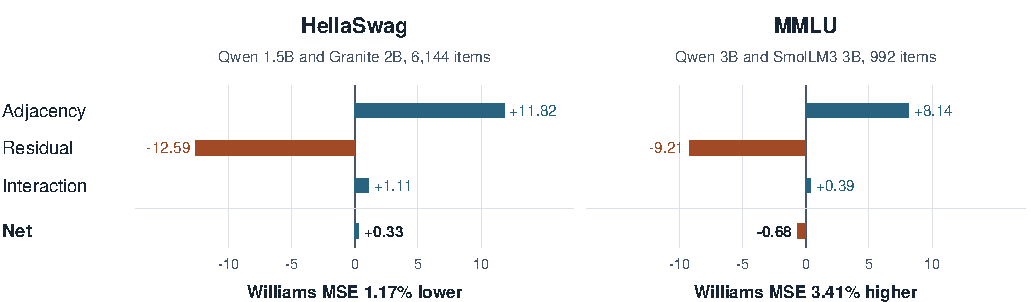
\includegraphics[width=\textwidth]{risk-components.pdf}
\caption{Exact risk accounting for HellaSwag and the frozen MMLU 3B
panel. Bars give contributions to precedence-minimax risk minus
Williams risk, averaged per item, in units of $10^{-3}$. Positive
values favor Williams. The percentages below the panels show the relative
change in MSE with Williams. Both comparisons use four shared orders per model and
question. The panels use different model pairs.}
\label{fig:risk-components}
\end{figure}

\section{Recorded scoring and outcome-independent gates}
\label{app:protocol}

\paragraph{OpenBookQA.}
The eligible source was the official four-option Main test split. The
192 IDs were selected by ascending SHA-256 of \texttt{221128:<id>}.
Each model saw the same 24 orders for each question with no examples
or retrieved facts. The native chat template was used with a single user
instruction and an explicit alphabetic label for each option. The
winner was the largest of four single-token label logits at the final
prompt position, with ties resolved toward the lower displayed position.
Inference used BF16 SDPA and left padding. The 9,216 model-item-order
records represent actual forward passes. The paired intervals used
2,000 bootstrap draws, stratified by original key, with seed 221129.
The paper's six point MSEs are calculated from binary correctness masks
and require no access to the model weights.

\paragraph{ARC-Challenge.}
The source-binding rule used the archive source index, official key and
the exact four choices, and excluded duplicate, ambiguous and previously
used items. An attempted literal-prompt check ended before scoring when
the author archive lacked those prompts. The subsequent frozen question
binding retained 1,154 items from 1,165 source-bound four-option records.
The position minimax gate required both full-order accuracies above 35\%,
at least 5\% point reduction and a positive lower 95\% bound versus all
balanced, and a lower 95\% gain bound of at least \(-10\%\) versus Williams.
Two arithmetic implementations independently matched the outcome.
The primary exact MSEs were \(1.49713\), \(1.63362\), and \(1.64470\),
in units of \(10^{-5}\), for Williams, all balanced and position minimax.

\paragraph{MMLU.}
Five previously used subjects were excluded before comparison. Two
source-only admissions stopped without parsing predictions, first on a
mismatched row and then on an unbindable subject. The final freeze
omitted both while retaining the same primary thresholds. Both models had to exceed 35\% full-order accuracy. The
comparison weights items equally, and the 8,000 paired bootstrap draws
resample whole subjects with seed 221151. Williams had to reduce MSE by at least 10\% versus ordinary
cyclic and 5\% versus all balanced and position minimax, have a positive
lower 95\% bound for each contrast, and win all three in at least two
thirds of the eligible subjects. The 5.09\% gain over all balanced meets
the point threshold, while the lower interval endpoint of 4.14\% still
admits a smaller gain. The evaluated archive supplies all 582,192
model-item-order records for the eligible cohort.

\section{HellaSwag confirmation protocol and results}
\label{app:hellaswag}
The 6,144 paired items were enrolled by committed within-stratum hash
order after excluding prior development and separately reserved records.
Both pinned model variants ran on the original RTX 4060 using llama.cpp
build b12631 and a cleared eight-sequence layout. Per item and model,
we saved scores for all 24 lexicographic orders and checked repeated
scores on the first eight orders. A failed resource guard interrupted
one attempt, which contributed zero accepted items. Its clean retry
and the other 15 shards supplied all \(294{,}912\) model-order cells.
Inference used 263.27 scoped GPU minutes and 265.46 CPU minutes, including
the failed attempt. The previous 192-item reserve remains separate.

At item level the practical contrast is \(0.95r_{i,C}-r_{i,W}\),
where \(r_{i,C}\) is the exact conditional block risk for design \(C\).
The primary interval uses the equally weighted mean of the two fixed
strata and sums their sample-variance terms with squared weights. Its
two-sided Bonferroni cutoff is the standard normal quantile
\(1-0.05/8\). The bounded sensitivity uses the prespecified
\([-1,0.95]\) item range and the same four-comparison family allocation.
Both intervals are divided by \(N\) to express the margin on the
benchmark MSE scale. Rule-out requires at least one strictly negative
upper endpoint, and support requires all four lower endpoints to be
strictly positive. The primary rule also requires nonzero estimated
variance for informative intervals. All four estimates here had
nonzero variance.

The five exact risks share denominator \(21{,}743{,}271{,}936\).
Their numerators are 99,719 (Williams), 105,647 (ordinary cyclic),
101,879 (all balanced), 102,479 (position minimax) and 100,895
(precedence minimax). The two all-order accuracies are
\(4069/9216\) and \(55883/147456\). The common bounded interval
half-width is approximately \(6.4501\times 10^{-6}\) benchmark MSE.
The matched exact and numerical receipts preserve all endpoints and
both decision outcomes. The all-order observations settle finite-panel
risks conditional on this prompt and model pair. The simultaneous
intervals address item-composition uncertainty under their respective
sampling assumptions.

\section{What the replay establishes}
\label{app:artifacts}

The compact OpenBookQA supplement contains a Python standard-library
enumerator, the two correctness masks per item, the original point-risk
reference, the exact integer output and a README. The arithmetic replay
regenerates the six point risks and the full-order accuracy gap without
network access. For example the two exact values underlying the cyclic
comparison are \(1157/21233664\) for Williams and \(1337/21233664\) for
ordinary cyclic. The capsule's SHA-256 is
\texttt{7995b53380266d76292dbae886bc2602fe04cd716453e86f5182b7b0fafd2c67}.
The original bootstrap and inference have separate dependencies.

ARC-Challenge and MMLU use the publisher's probability exports,
which can be retrieved at revision
\texttt{29fcbb4807bc53a84ac26a64ddbad9526c940958} of
\href{https://github.com/chujiezheng/LLM-MCQ-Bias_data/tree/29fcbb4807bc53a84ac26a64ddbad9526c940958}{the original scorer archive}.
The source-bound replays require verified official question files,
the relevant archive blobs and the corresponding roster and analysis.
Independent integer checks reproduced all primary point risks given those
inputs. The original prompts are unavailable. The archive verifiers and
frozen manifests are separate from the OpenBookQA supplement.

\section{Additional full-order comparisons}
\label{app:other-panels}
An archived development study used 7,600 AG News items and three
models \citep{gao2026}. Its registered double-transposition proposal
reduced MSE by 4.70\% versus ordinary cyclic, below its 10\% gate.
Williams had 11.75\% lower MSE in a descriptive comparison. That
finding motivated the independent design test.

\paragraph{Fresh OpenBookQA.}
Before inference we selected 192 official test IDs \citep{mihaylov2018} without using their
answer labels and fixed the two models, common prompt, single-token
option-label scoring, matched orders and analysis. The Qwen2.5-0.5B-Instruct
and SmolLM2-360M-Instruct checkpoints were absent from the development
panel. The gate required reductions of at least 10\% versus ordinary cyclic
and 5\% versus reversal pairs, positive lower paired intervals for both,
and nonnegative gains over the other prespecified controls.
Table~\ref{tab:obqa} reports the complete set. The full-order accuracies
were 27.50\% and 25.91\%, and gap RMSE was 0.738 percentage points with
Williams and 0.794 with ordinary cyclic. The gate passed on this
low-capacity model pair.

\begin{table}[t]
\caption{OpenBookQA exact gap MSE in units of $10^{-5}$. Relative
reductions are for Williams versus each comparator. The paired intervals
resample items and hold the model responses fixed.}
\label{tab:obqa}
\centering
\small
\setlength{\tabcolsep}{4pt}
\begin{tabular}{@{}lrr@{}}
\toprule
Design & MSE & Gain [95\% interval] \\
\midrule
Williams & 5.449 & --- \\
Ordinary cyclic & 6.297 & 13.46 [3.32, 23.59] \\
Reversal pairs & 27.022 & 79.84 [74.48, 84.48] \\
Uniform four & 25.246 & 78.42 [73.02, 83.29] \\
Double transpos. & 6.240 & 12.68 [3.74, 21.77] \\
All balanced & 5.915 & 7.88 [0.48, 15.72] \\
\bottomrule
\end{tabular}
\end{table}

\paragraph{Source-bound ARC-Challenge.}
We evaluated the strict position minimax policy on a separately frozen
historical zero-shot full-order archive \citep{zheng2024,clark2018}.
Official keys, options and row identity checks retained 1,154 items.
An independent implementation reproduced 2,330 author aggregate labels
and matched exact risks. Llama-2-70B-chat and Falcon-40B-instruct had full-order accuracies of
77.78\% and 61.09\%. Strict minimax had 0.68\% higher MSE than all balanced
blocks (95\% gain interval $[-1.51,0.21]$) and 9.86\% higher MSE than
Williams (gain interval $[-14.27,-5.63]$). These results missed the
joint gate, including an interval-based 10\% noninferiority requirement
against Williams.

\paragraph{Cross-subject MMLU.}
Before parsing model outcomes, eligibility checks required exact source
binding to official questions \citep{hendrycks2021}. Five previously
opened subjects were held out of the analysis. We excluded one
mismatched row and a subject whose generic options and keys could not
identify rows. The 12,129 eligible items cover 51 subjects.
Vicuna-33B-v1.3 and Falcon-40B base reached 59.55\% and 53.13\%,
respectively, averaged over all orders. The replay reproduced 25,266
archive aggregate labels and independently matched all primary exact
risks. Williams cleared the frozen joint gate. All three primary
gains were positive in 45 subjects. The descriptive comparison with
precedence minimax is inconclusive (Table~\ref{tab:mmlu}).

\begin{table}[t]
\caption{MMLU relative risk reduction for Williams. Paired 95\%
intervals resample subjects and hold checkpoints and archived
responses fixed.}
\label{tab:mmlu}
\centering
\small
\begin{tabular}{lrr}
\toprule
Comparator & Reduction (\%) & 95\% interval \\
\midrule
Ordinary cyclic & 15.93 & [14.36, 17.76] \\
All balanced & 5.09 & [4.14, 6.10] \\
Position minimax & 6.12 & [5.14, 7.21] \\
Precedence minimax & 0.30 & [$-0.46$, 1.07] \\
\bottomrule
\end{tabular}
\end{table}

\section{Development Diagnostics}
On previously opened SciQ and ARC-Easy items, a Q4\_K\_M Qwen2.5 3B
and SmolLM3 3B engineering pilot scored 32 questions per benchmark
with standard and direct prompts. Across these four panels the
all-order gap ranged from 49.22 to 58.33 percentage points. Exact
convolution gave zero rank reversals for each tested design. These
large gaps offer little information about decisions between closely
matched models. Replaying eight SciQ items on a second GPU changed
18 of 384 displayed answers across the two models. Two cold replays
on the original GPU matched the original choices in all 1,536
checked model--item--order cells per replay. In the opened 480-item
SciQ panel for Qwen2.5 1.5B and Granite 3.3 2B, the reference
gap was 4.24 points. If an evaluator requires a lead of at least
five percentage points, the four-order estimate crosses that
threshold in 9.08\% of Williams draws, 9.27\% of precedence-minimax
draws and 11.17\% of ordinary cyclic draws. These probabilities
condition on the observed response profiles.

A separate four-panel development screen used 48 full-order items
per panel to estimate risk by projecting paired disagreement onto
position, precedence and directed-adjacency components. Against the
fixed comparator selected on calibration, four-call gains ranged
from $-1.59$\% to $+0.70$\%. With calibration charged and the same
total calls available to the fixed comparator, the adaptive rule
increased MSE by 48.96--52.39\%. This screen does not advance the rule
to confirmation.


\paragraph{Scope of the additional panels.}
OpenBookQA's independent scoring protocol uses two near-chance small
models. The larger HellaSwag confirmation adds a distinct numeric-choice
prompt and model pair. ARC-Challenge and MMLU use different above-chance
pairs with the same archival scoring convention. The historical release
lacks literal prompts. Exact replay establishes arithmetic reproducibility
and source binding for those archives. Prompt, tokenizer, checkpoint,
and quantization all constrain interpretation.
An earlier RACE \citep{lai2017} transfer attempt stopped on its first
numerical cache check and yielded zero validated model-items.

The bootstrap intervals quantify sensitivity of empirical MSE rankings
to item or subject composition. They differ from uncertainty for the
gap when only four calls per model are made. A spent-panel development
replay found conservative finite-panel bounds using squared differences
between independent item blocks 31.44\% and 16.43\% narrower than
the strongest tested nonpaired bounds on OpenBookQA and ARC-Challenge.
Random pairing performed similarly. Across 4,096 draws at each of
0-, 1- and 5-point margins, every method left OpenBookQA unresolved and
certified ARC-Challenge. The interval method has no independently
validated transfer or measured decision advantage in these panels.
